\section{Protocolo de transmisión}
	\subsection{Descripción del problema}
	Desarrollar un programa que genere 50 cadenas de 32 caracteres que sean guardadas en un archivo, para después ser evaluadas por un autómata, en este caso el de paridad binaria y guardar las cadenas binarias validas en otro archivo, siguiendo el siguiente diagrama.
	\begin{figure}[H]
		\begin{center}
			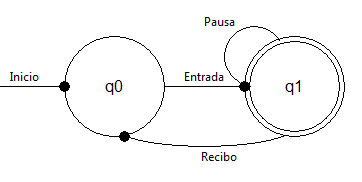
\includegraphics[width=10cm, height=5cm]{img/protocolo.png}
			\caption{Diagrama de transiciones del autómata. \cite{WEB}}
			\label{fig:diagrama3}
		\end{center}
	\end{figure}
	\subsection{Código}
	El código fue realizado en Python 3.5.
	\subsection{Pruebas}
	Pruebas de las opciones del menú.
	{\large Modo automático.}
	\begin{figure}[H]
		\begin{center}
			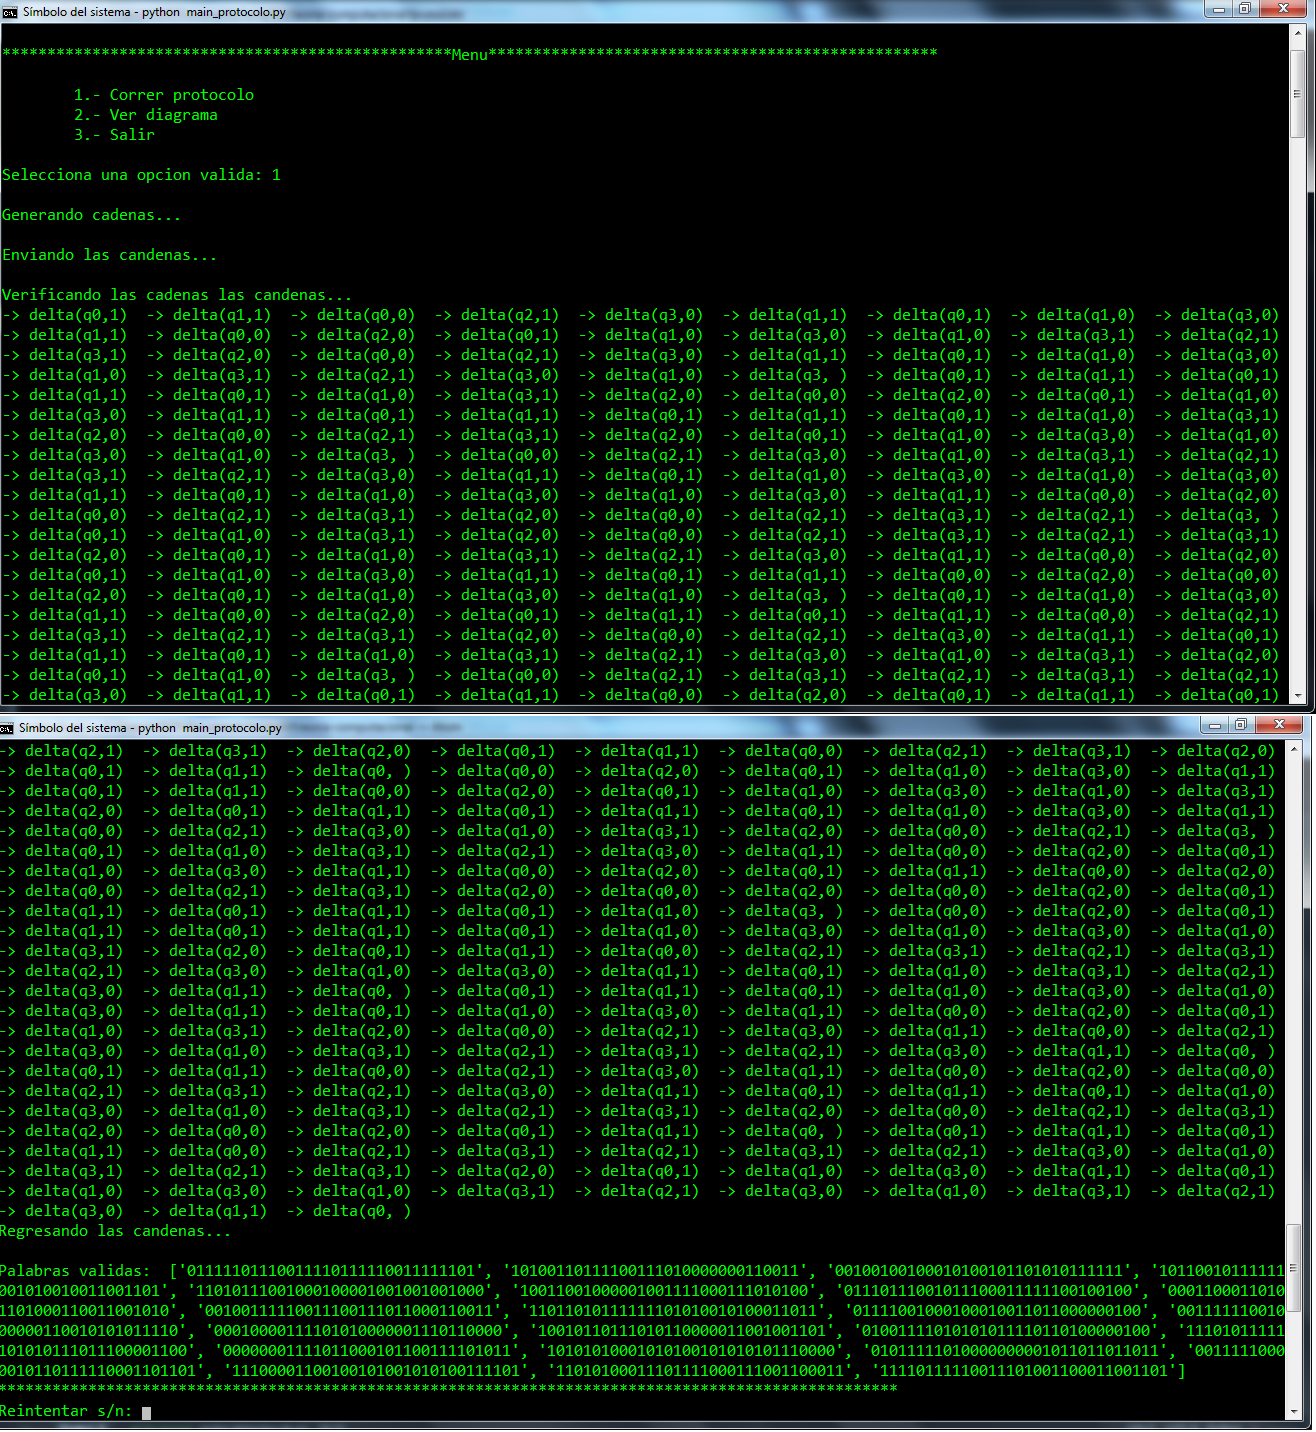
\includegraphics[width=10cm, height=5cm]{img/protocolo-automata.png}
			\caption{Historia del protocolo. \cite{WEB}}
			\label{fig:protocolo1}
		\end{center}
	\end{figure}
	\begin{figure}[H]
		\begin{center}
			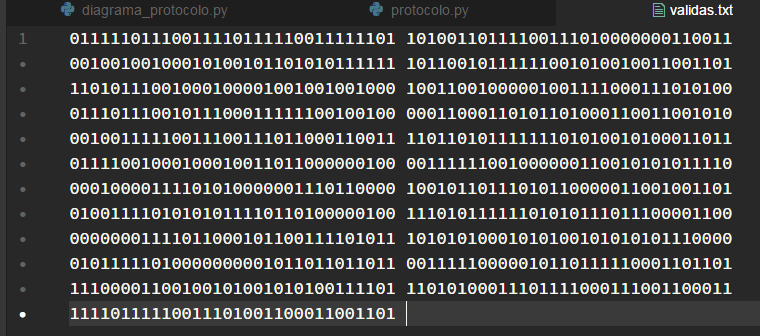
\includegraphics[width=10cm, height=5cm]{img/protocolo-salida.png}
			\caption{Palabras validas. \cite{WEB}}
			\label{fig:protocolo2}
		\end{center}
	\end{figure}
	{\large Diagrama.}
	\begin{figure}[H]
		\begin{center}
			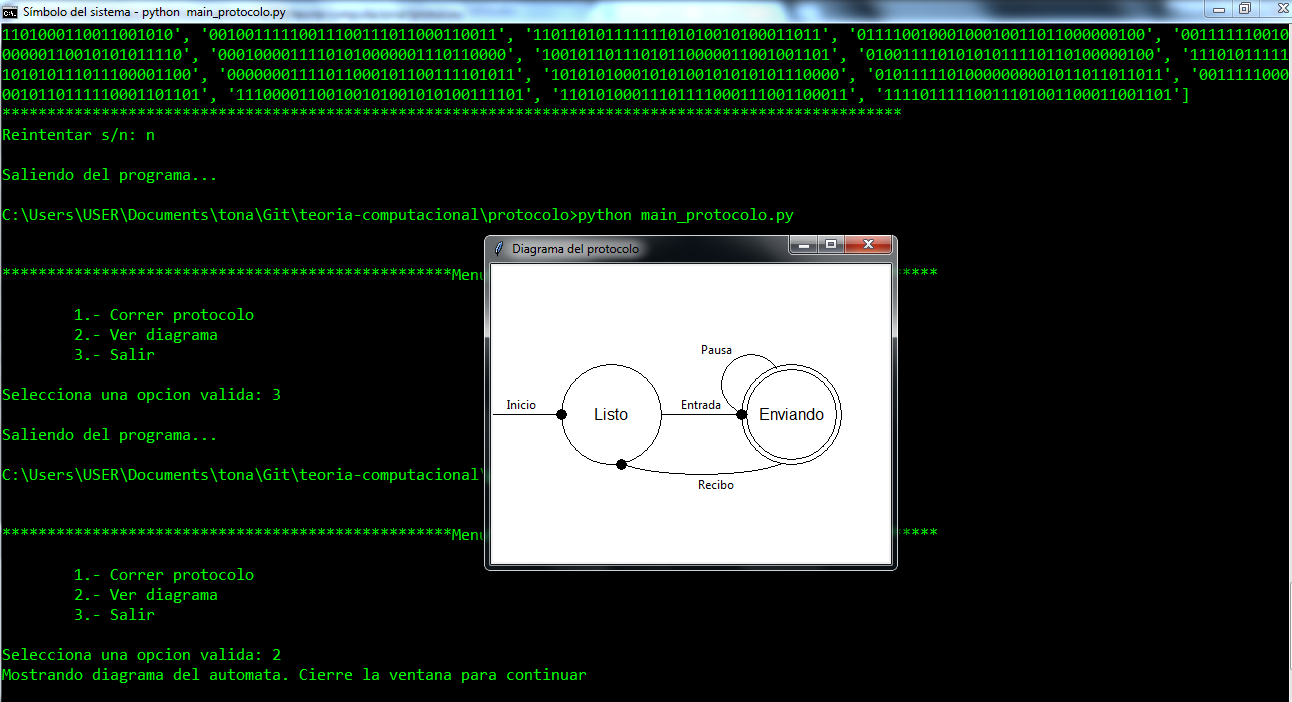
\includegraphics[width=10cm, height=5cm]{img/protocolo-diagrama.png}
			\caption{Diagrama de transiciones del autómata.}
			\label{fig:protocolo3}
		\end{center}
	\end{figure}